\begin{Schunk}
\begin{Sinput}
> library("Ham94", lib.loc = "../../../library")
\end{Sinput}
\end{Schunk}
Page 3 describes calculations for dynamic multipliers for first order difference equations.  An example of these
calculations in action is given on page 4.  A simple method to calculate dynamic multipliers is to simulate
the difference equation calculating forward based on an initial shock at time t=1, assuming the value of y at time 0 is 0.
R indexes arrays starting at 1 instead of 0, so subscripts are one more than the convention used in the text, meaning that
the shock will be said to occur at time 2.
\begin{Schunk}
\begin{Sinput}
> T <- 20
> w <- 1 * (1:T == 2)
\end{Sinput}
\end{Schunk}
In the examples shown on page 4 there are actually four different equations being simulated,
so we will use a matrix, rather than a vector, to store the results.
\begin{Schunk}
\begin{Sinput}
> phis <- c(0.8, -0.8, 1.1, -1.1)
> y <- array(dim = c(T, length(phis)))
> y[1, ] <- rep(0, length(phis))
> for (j in 2:T) y[j, ] <- phis * y[j - 1, ] + w[j]
\end{Sinput}
\end{Schunk}
We can check this calculation against the closed form expression on page 3.
\begin{Schunk}
\begin{Sinput}
> print(y[2:T, 1])
\end{Sinput}
\begin{Soutput}
 [1] 1.00000000 0.80000000 0.64000000 0.51200000 0.40960000 0.32768000
 [7] 0.26214400 0.20971520 0.16777216 0.13421773 0.10737418 0.08589935
[13] 0.06871948 0.05497558 0.04398047 0.03518437 0.02814750 0.02251800
[19] 0.01801440
\end{Soutput}
\begin{Sinput}
> print(phis[[1]]^seq(0, T - 2))
\end{Sinput}
\begin{Soutput}
 [1] 1.00000000 0.80000000 0.64000000 0.51200000 0.40960000 0.32768000
 [7] 0.26214400 0.20971520 0.16777216 0.13421773 0.10737418 0.08589935
[13] 0.06871948 0.05497558 0.04398047 0.03518437 0.02814750 0.02251800
[19] 0.01801440
\end{Soutput}
\end{Schunk}
Finally we can plot the results using a histogram plot reproducing figure 1.1.
\begin{center}
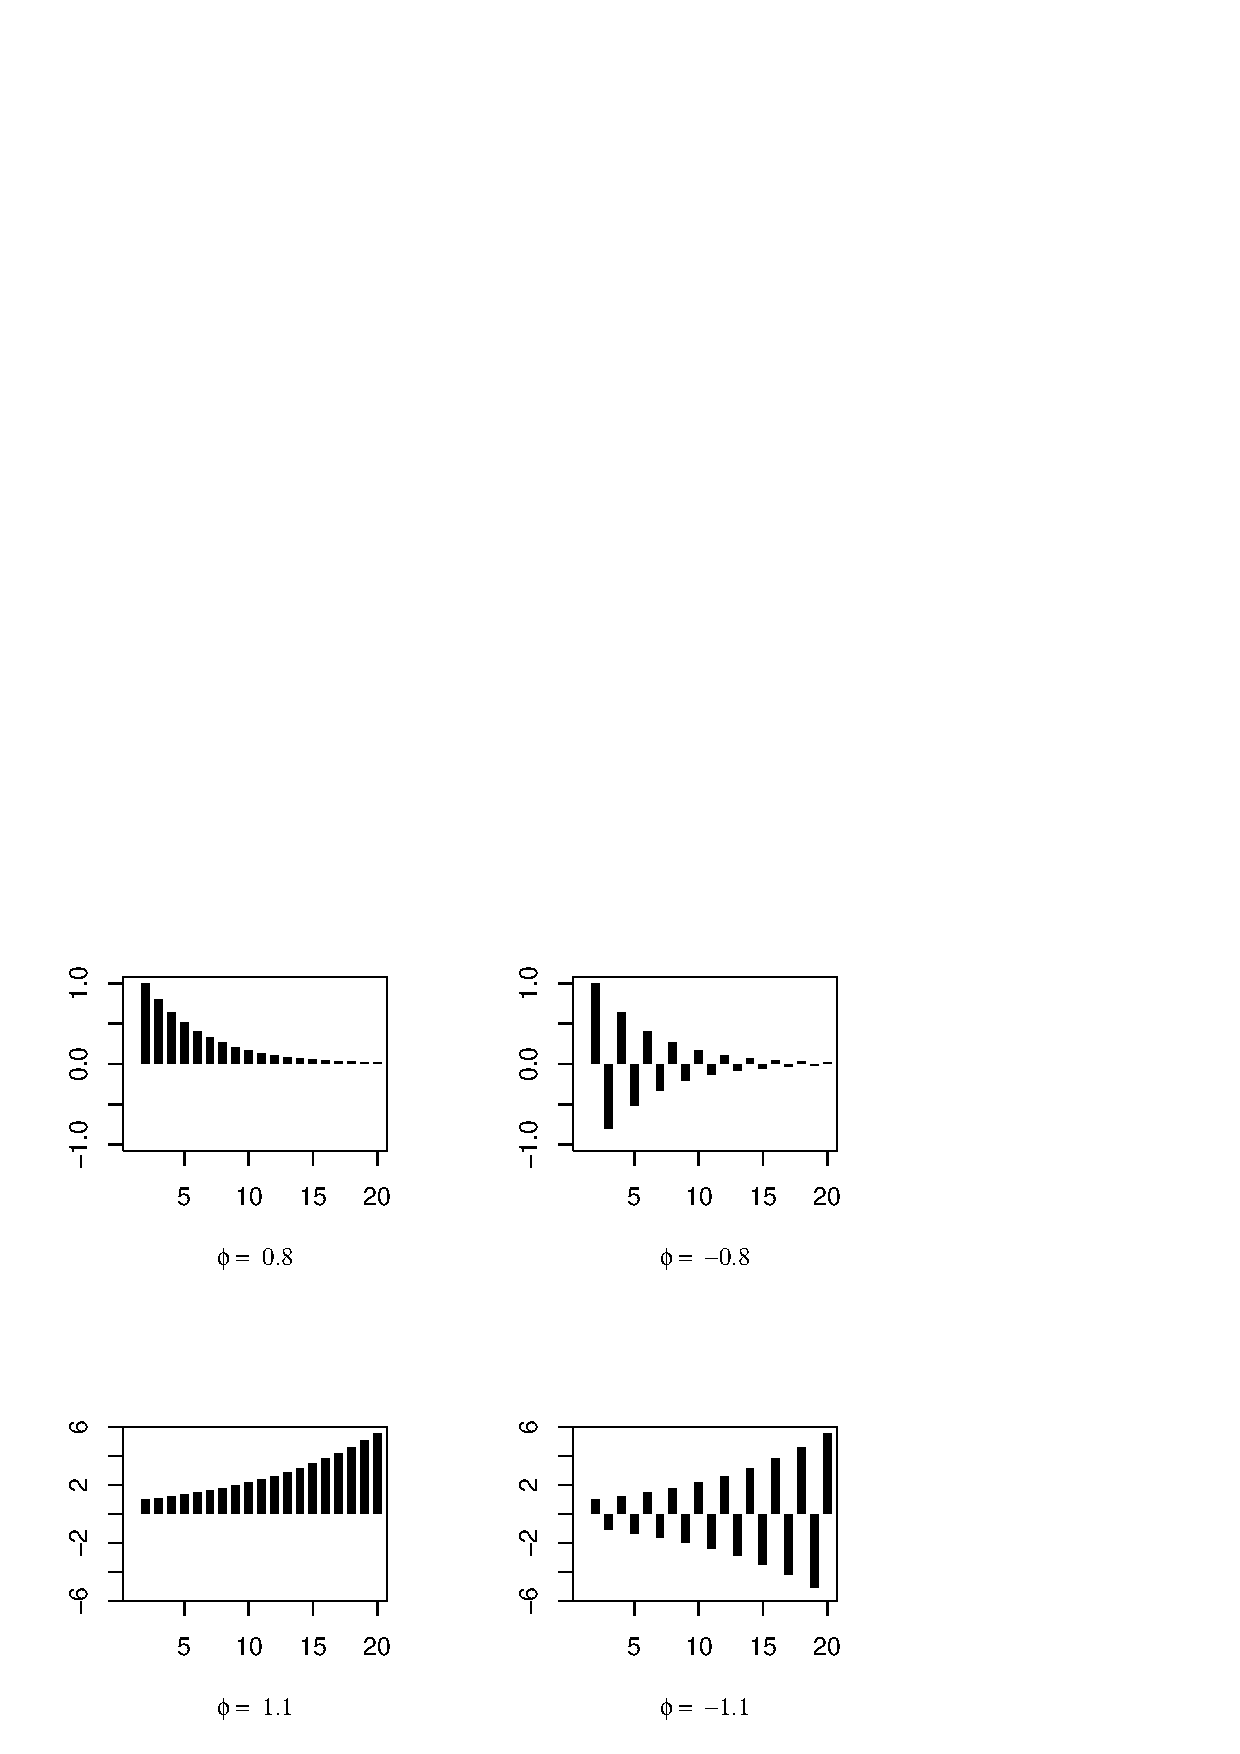
\includegraphics{p4-005}
\end{center}
